\section{Исследовательский раздел}

\subsection{Технические характеристики}

Технические характеристики устройства, на котором выполнялись замеры, следующие.

\begin{itemize}[label=---]
	\item Операционная система Windows 10 \cite{oswind} x86\_64.
	\item Память 8 Гб 2400 МГц DDR4.
	\item 1.6 ГГц 4-ядерный процессор Intel Core i5 8265U \cite{intel}.
\end{itemize}

Замеры проводились на ноутбуке, включенном в сеть электропитания. Во время проведения исследований ноутбук был нагружен только встроенными приложениями окружения, а также непосредственно системой выполнения замеров.

\subsection{Подготовка исследования}

Для сравнения производительности разработанного сервера с nginx необходимо установить утилиту для нагрузочного тестирования Apache Bench-\\mark~\cite{ab}. Данный инструмент позволяет исследовать допустимые границы количества запросов, которое сервер может обработать в секунду.

Также необходимо настроить nginx~\cite{nginx} на отдачу статического контента. Конфигурация nginx представлена в листинге \ref{nginx}.

\begin{lstlisting}[caption={Конфигурация nginx}, label=nginx]
worker_processes  5;
pid        /var/run/nginx.pid;
error_log  /var/log/nginx/error.log info;

events {
\end{lstlisting}

\begin{lstlisting}[title={Окончание листинга \ref{nginx}}, label=nginx1, firstnumber=6]
  worker_connections  4096; 
}

http {
charset utf-8;

server { 
	location / {
		include  /etc/nginx/mime.types;
		# don't cache it
		proxy_no_cache 1;
		# even if cached, don't try to use it
		proxy_cache_bypass 1; 
		root /static;
	}
	
	location /status {
		stub_status;
	}
}
}
\end{lstlisting}

Для запуска nginx используется Docker~\cite{docker}. Содержимое используемого файла docker-compose.yml представлено в листинге \ref{compose}.

\begin{lstlisting}[caption={Конфигурация docker-compose.yml}, label=compose]
version: '3.7'
services:  
  nginx:
  image: nginx
  volumes:
    - ./logs:/var/log/nginx
    - ./nginx.conf:/etc/nginx/nginx.conf
    - C:\Users\Pavel\Desktop\parcorpus\static:/static
\end{lstlisting}
    
\begin{lstlisting}[title={Окончание листинга \ref{compose}}, label=compose1, firstnumber=9]
  ports:
    - "80:80"
    - "443:443"
  restart:
    always
\end{lstlisting}

\subsection{Результаты замеров}

Замеры проводились для двух файлов: для jpg-файла размером 53 Кб и pdf-файла размером 2.11 Мб. Были произведены замеры при постоянном числе запросов 10000 для jpg-файла и 1500 для pdf-файла и изменяющимся максимальным числом конкурентных запросов. На рисунках \ref{jpg-comparison-c} и \ref{pdf-comparison-c} представлена зависимость числа RPS (англ. requests per second -- числа запросов в секунду) от числа конкурентных запросов для jpg и pdf файлов соответственно.

\captionsetup{singlelinecheck = false, justification=centering}
\begin{figure}[H]
	\centering
	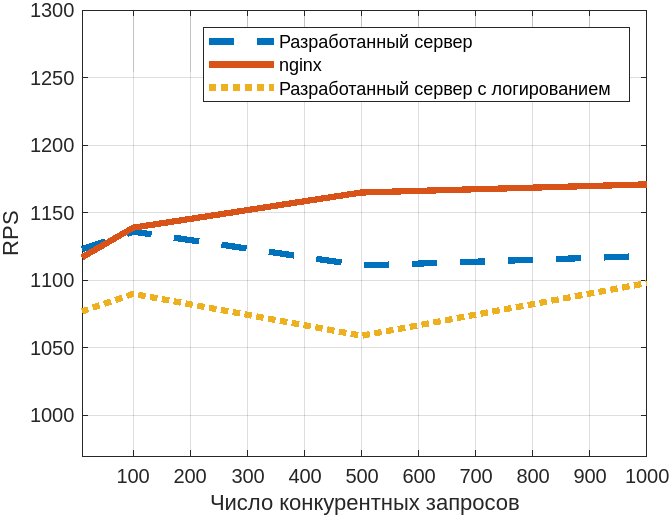
\includegraphics[scale=1.1]{img/jpg-c.png}
	\caption{Зависимость RPS от числа конкурентных запросов (jpg)}
	\label{jpg-comparison-c}
\end{figure}

\captionsetup{singlelinecheck = false, justification=centering}
\begin{figure}[H]
	\centering
	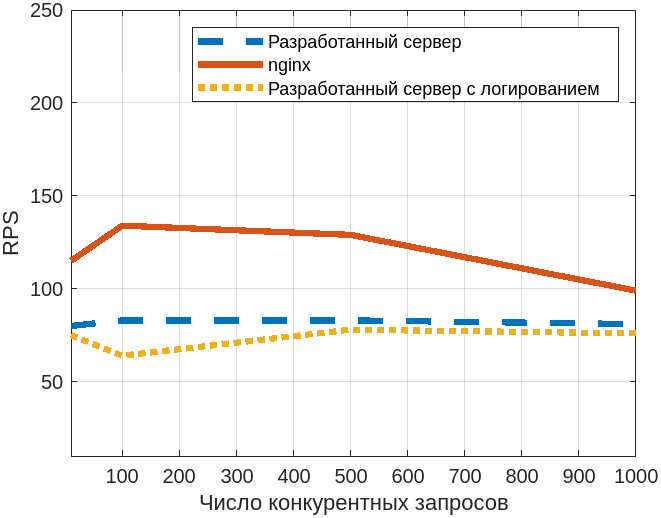
\includegraphics[scale=1.1]{img/pdf-c.png}
	\caption{Зависимость RPS от числа конкурентных запросов (pdf)}
	\label{pdf-comparison-c}
\end{figure}

\subsection*{Вывод}

В результате проведенных замеров установлено, что разработанный сервер работает, как правило, медленнее, чем nginx. Время ответа на запросы разработанным сервером в 1.05 -- 1.54 раза больше. Это может быть связано с тем, что nginx -- более оптимизированное программное обеспечение, предназначенное для профессионалов~\cite{nginx-tuning}, а также оптимизацией сторонних процессов, таких как логирование и мониторинг дочерних процессов.

Однако нагрузочное тестирование показало, что сервер работает стабильно: программа корректно обработала все запросы, посылаемые ей в рамках исследования.

\pagebreak